The identification of rich wind resources have become important together with the increasing focus on green energy \cite{WindPowerGenerationUsingANN}. It can come as no surprise that the meteorological factors like wind speed and air density have a huge impact on the wind power generation. Figure~\ref{fig:energyGeneration} shows how the monthly energy generation increases with the monthly average wind speed. 

\begin{figure}[h!]
\centering
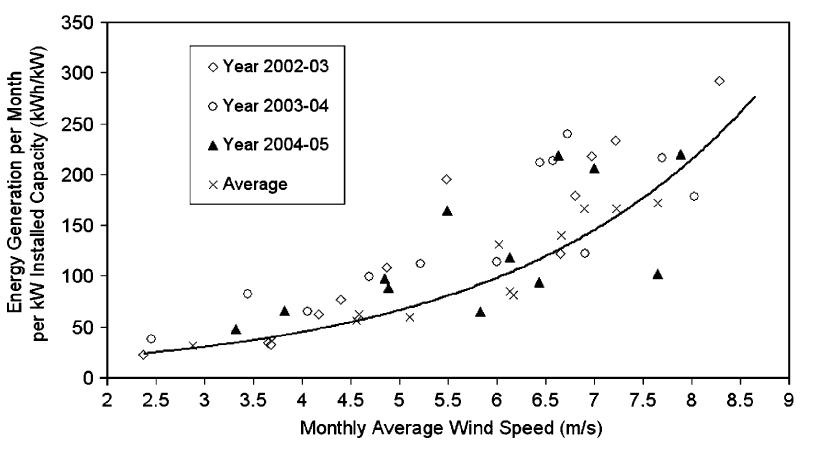
\includegraphics[width=0.8\linewidth,natwidth=898,natheight=587]{billeder/EnergyGenerationVsWindSpeed.png}
\caption{The influence of wind speed on the energy generation \cite{WindPowerGenerationUsingANN}}
\label{fig:energyGeneration}
\end{figure} 

\subsubsection{Windmill Placement}
It is important to analyse and predict the wind power generation at a certain location before placing actual windmills. Before investing billions of dollars in a new wind farm it is of utmost importance to put it in the best possible location in relation to wind statistics, e.g. force of the wind and how often the winds change in power and direction at the position. In \cite{4} they use a Measure-Correlate-Predict (MCP) method to predict wind statistics based on large amount of geographical-, weather- and historical data so that the farms can be placed best possible. These algorithms are heavy and will do calculations on sensor data directly from the location for months before giving any results. Time is not an issue because the the company need to know for certain that the location will make the wind mills produce to the best or their ability.

Another approach is seen in \cite{WindPowerGenerationUsingANN} where wind speed, relative humidity and generation hours of the windmills are used as input for an Artificial Neural Network. The more "heavy" the air, the more energy is received by the windmill turbine. The humidity increases as air density increases and because wind energy is proportional to air density the prediction algorithm needs humidity as input because it also accounts for temperature and pressure \cite{AirDensityInForecast}. Moist air is lighter than dry air because water molecules are less dense than the molecules in dry air such as oxygen and nitrogen. This basically means that the more air molecules like oxygen and nitrogen the more wind energy.

The last parameter in their prediction algorithm is generation hours which is the period in which the turbines produce power. The number of hours are influenced by f.x mechanical breakdowns, scheduled maintenance and low wind speeds. It is clear that the more generation hours the more energy is produced as seen in figure ~\ref{fig:energyGenerationFromHours}. The generation hours are hard to predict but can be calculated from past years up-time together with the expectations of the company delivering the windmills.  

\begin{figure}[h!]
\centering
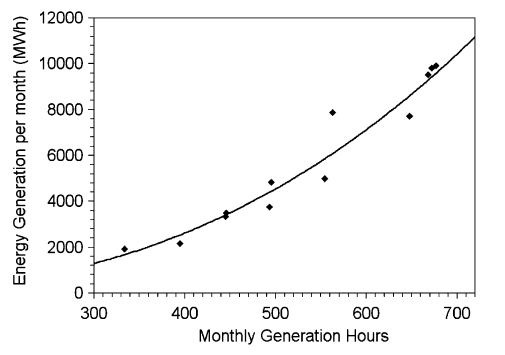
\includegraphics[width=0.8\linewidth,natwidth=898,natheight=587]{billeder/GenerationHourVSGeneration.png}
\caption{The influence of generation hours on energy production \cite{WindPowerGenerationUsingANN}}
\label{fig:energyGenerationFromHours}
\end{figure} 

The Artificial Neural Network trains 3-year dataset containing the mentioned input parameters. The input parameters are during the training compared to the output variable which is the wind energy output of the turbine. See figure~\ref{fig:annArchitecture} for the architecture.
\\[0.5cm]
\begin{figure}[h!]
\centering
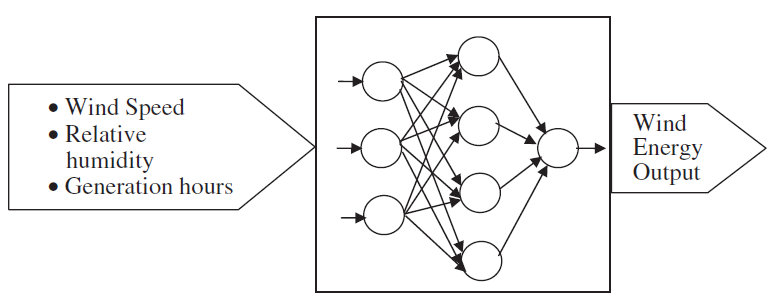
\includegraphics[width=0.7\linewidth,natwidth=898,natheight=587]{billeder/ANNwindSpeedPrediction.png}
\caption{Artificial Neural Network architecture from \cite{WindPowerGenerationUsingANN}}
\label{fig:annArchitecture}
\end{figure}

\subsubsection{Nearest Neighbour Approach}
Prediction can be done by using an algorithm that produces weighted nearest-neighbour tables to generate wind power curves based on available wind speed and direction from an online weather-data source. The weighted approach allows the algorithm to adapt to seasonal changes by weighting newest results highest, and the power curves makes it possible to use the algorithm on different wind farms. This prediction is used to schedule jobs in data centers which is described in the related work section.

The time perspective and data of the algorithm is comparable to our specific purpose. The ANN prediction will need to fetch data from online sources but it will also be based on a great deal of historical data to achieve higher accuracy. Furthermore, the algorithms use is different from what is presented in the thesis. 

\subsubsection{Summary}
It is described how the weather influence the wind power production and exactly what parameters are necessary to consider when doing the prediction. An Artificial Neural Network for prediction of wind power is presented and they discuss the concept of generation hours. It is necessary to investigate how the generation hours of the wind mills can be calculated or estimated because it will result in better production forecasts. 

Furthermore, examples of how these predictions are used today is described. They are mainly used for placement planning of wind mill farms. Some knowledge can be transferred to our specific purpose but decision making in real-time cannot rely on heavy algorithms that will do calculations for months and years on data directly from the location. We must deliver accurate estimates without delaying the trader's work. 